\clearpage
\section*{Figure titles and legends}
\addcontentsline{toc}{section}{Figure titles and legends}

\refstepcounter{figure}\label{fig:fig1}
\noindent\textbf{Figure 1.} \textbf{HistoAtlas converts routine pathology into a named, 
compartment-resolved measurement layer.} 
(A)~Pipeline, illustrated on one lung adenocarcinoma slide (TCGA-MP-A4T9). 
Diagnostic H\&E whole-slide images (\num{6745} slides from \num{6088} patients, 
21 TCGA cancer types) are segmented into tissue compartments and spatial bands 
and into individual cells (H\&E tile and cell-call overlay, 224 $\times$ 224 
pixels), from which 38 measurements in six groups are computed per slide. A 
statistical layer links each measurement to outcomes and molecular data, and 
the results are served through a web atlas and a programmatic interface 
(screenshot of the atlas). This panel is an explanatory schematic composed in 
Claude Design (Anthropic) from pipeline images that were not altered. 
(B)~Spearman correlation between the 38 measurements across all slides with 
complete measurements ($n = \num{5916}$), ordered by Ward-linkage clustering 
(dendrogram above). The diagonal is masked; the strip beside each row gives the 
measurement group. 
(C)~UMAP embedding of all \num{6745} slides colored by cancer type, with 
kernel-density contours (gray) and labels at the median position of the larger 
cancer types. The embedding is used for display only. 
(D)~Cancer-type composition of the ten pan-cancer $K$-means clusters (slides per 
cluster in parentheses); types making up at least 20\% of a cluster are labeled. 
The right column gives the overall-survival hazard ratio of cluster membership 
where significant (Cox regression stratified by cancer type, 
Benjamini--Hochberg adjusted $P < 0.05$; down triangle, lower hazard; up 
triangle, higher hazard; dash, not significant). 
(E)~Mean $z$-scored measurement value per cluster (rows ordered as in D), 
clipped at $\pm 2$; measurements are ordered by Ward-linkage clustering and the 
strip above gives the measurement group.
\par\medskip

\refstepcounter{figure}\label{fig:fig2}
\noindent\textbf{Figure 2.} \textbf{Six continuous histomic programs summarize the measurement 
space and partially transfer across cohorts.} 
(A)~Sparse principal component loadings of the 38 measurements on six programs, 
fitted on \num{5371} TCGA patients with complete measurement vectors 
($\alpha = 1.0$). Measurements are grouped by the program on which they load 
most strongly. Program names summarize the pathway correlations in (C). 
(B)~Distributions of program scores in TCGA (blue, $n = \num{5371}$) and in 
CPTAC after projection with the unchanged TCGA-fitted transform (orange, 
$n = 297$). Violins are kernel density estimates; boxes show the interquartile 
range, the white line the median and whiskers the 5th to 95th percentiles. 
$D$ and $P$, two-sample Kolmogorov--Smirnov test. 
(C)~Spearman correlation between each program and each of the 50 MSigDB 
Hallmark pathway activity scores in TCGA ($n = \num{5371}$), pathways ordered by 
Ward-linkage clustering. Dots mark Benjamini--Hochberg adjusted $P < 0.05$ 
across the 300 tests.
\par\medskip

\refstepcounter{figure}\label{fig:fig3}
\noindent\textbf{Figure 3.} \textbf{Compartment-resolved immune topology is prognostic and 
molecularly anchored.} 
(A)~Hazard ratios for overall survival per standard deviation of intratumoral 
(blue circles) and stromal (orange diamonds) lymphocyte density, from Cox models 
adjusted for age, sex and pathologic stage and stratified by tissue source site 
(pan-cancer models additionally stratified by cancer type). Lines are 95\% Wald 
confidence intervals, truncated at the axis limits. Filled markers denote 
moderate or strong evidence badges; open markers suggestive or insufficient 
evidence. Cancer types without a valid adjusted model for either measurement 
(PRAD, THYM, UCS) are omitted; $n$, patients per model. 
(B)~Kaplan--Meier estimates of overall survival in breast carcinoma for patients 
above and below the median intratumoral lymphocyte density ($n = 480$ each; 
shaded bands, 95\% confidence intervals; ticks, censoring), with numbers at risk 
below. The hazard ratio shown is from the adjusted Cox model on the continuous 
measurement, not from the dichotomized groups. 
(C)~Tumor--lymphocyte nearest-neighbor distance at the invasive front against 
\textit{CD8A} expression in breast carcinoma, both as percentile ranks 
($n = 958$ patients). The line is the least-squares fit on ranks, whose slope 
equals Spearman $\rho$. Statistics are from the unadjusted model; Spearman 
correlation with analytical $t$-approximation $P$ value, Benjamini--Hochberg 
adjusted within its declared family; 95\% bootstrap confidence interval. 
(D)~The ten strongest positive and five strongest negative gene correlates of 
intratumoral lymphocyte density among significant associations in breast 
carcinoma ($n = 953$, adjusted for age). Bars are Spearman $\rho$, error bars 
95\% bootstrap confidence intervals (\num{1000} resamples); immune-checkpoint 
genes are in bold.
\par\medskip

\refstepcounter{figure}\label{fig:fig4}
\noindent\textbf{Figure 4.} \textbf{The measurement layer and its molecular links transfer to an 
independent consortium and extend to protein.} 
(A)~Standardized difference for each measurement and matched cancer type, 
computed as (median in CPTAC $-$ median in TCGA) / standard deviation in TCGA 
over all slides of that type (CPTAC $n$: BRCA 198, HNSCC 390, LUAD 240, PAAD 175, 
UCEC 92; TCGA $n$: 1,037, 471, 511, 146, 459). Dots mark $|d| > 1$; the numbers 
above each column count measurements with $|d| \leq 1$ (prespecified pass, 
$\geq 31$ of 38). Rows follow the measurement groups (strip, colors as in 
Figure~\ref{fig:fig1}). 
(B)~Spearman coefficients of the same measurement--gene pairs (expression, 
unadjusted) in TCGA and CPTAC, across all \num{25155} pairs evaluable in both 
cohorts, shown as a two-dimensional histogram (log color scale); dashed line, 
identity; $r$, Pearson correlation across pairs. 
(C)~Messenger RNA versus protein Spearman coefficients for the same measurement 
and gene in the four CPTAC cancer types with proteomics ($n = \num{14687}$ 
pairs, histogram as in B). Orange points are the 320 pairs significant in both 
modalities, of which 316 have the same sign (98.8\%, 95\% Clopper--Pearson 
interval 96.8\% to 99.7\%). 
(D)~Evidence triangulation for representative measurement--gene pairs grouped 
by biological axis. A filled circle denotes significance (false discovery rate 
below 0.05) in at least one cancer type for TCGA messenger RNA, CPTAC messenger 
RNA and CPTAC protein; the survival column marks a significant 
overall-survival association of the measurement itself in TCGA (unadjusted 
model) and is therefore shared by all genes of an axis. Open circles denote 
non-significance, which for CPTAC frequently reflects limited power rather than 
a contradicted effect.
\par\medskip

\refstepcounter{figure}\label{fig:fig5}
\noindent\textbf{Figure 5.} \textbf{Histomic measurements add a small increment beyond bulk 
molecular measurements.} 
(A)~Overall-survival hazard ratios (95\% confidence intervals) before (blue 
circles; age, sex and, where available, stage) and after (orange triangles) 
adding matched molecular covariates: \textit{CD8A}, \textit{TIGIT}, immune 
subtype and leukocyte fraction for the two immune measurements; 
\textsc{hallmark\_g2m\_checkpoint} and \textit{MKI67} for mitotic index. For 
each measurement, the cancer type with the strongest clinical-model association 
is shown; $n$, patients. 
(B)~Harrell's concordance index of four nested Cox models in breast carcinoma 
($n = 940$, 127 events): clinical covariates only, plus the matched transcript 
(named at left), plus the measurement, and plus both. Values are apparent 
(in-sample) concordance. 
(C)~Spearman correlation between each measurement and each protein before 
(horizontal axis) and after (vertical axis) partialling out the matched 
transcript, for \num{14686} triplets with both values in four CPTAC cancer types 
(two-dimensional histogram, log color scale; dashed line, identity). Orange 
points are the 132 triplets that remain significant after adjustment 
(Benjamini--Hochberg per cancer type; 120 in breast carcinoma); 77\% of 
triplets retain more than half of their unadjusted magnitude.
\par\medskip

\refstepcounter{figure}\label{fig:fig6}
\noindent\textbf{Figure 6.} \textbf{From cohort statistics back to cells: spatial provenance in 
HistoAtlas.} 
(A)~Tissue compartment map of a breast carcinoma slide (TCGA-A1-A0SE) showing 
the spatial bands defined by the signed distance to the tumor boundary; the 
pipeline's label colors were remapped to the palette shown. Circles mark the 
three highest-scoring tiles for intratumoral (blue, 1) and stromal (orange, 2) 
lymphocyte density; the largest circle marks the top tile. 
(B)~The two overall-survival associations that a user reaches from this slide 
(adjusted Cox models in breast carcinoma, $n = 960$, 135 events; hazard ratio 
per standard deviation with 95\% confidence interval). 
(C and D)~The three highest-scoring $224 \times 224$ pixel tiles on this slide 
for intratumoral (C) and stromal (D) lymphocyte density, as H\&E (top) and with 
the cell calls of the cell model outlined (bottom), with the tile score used to 
rank them. Images are the atlas's own tiles, shown unaltered. Lymphocyte calls 
(green outlines) dominate the two top-ranked tiles of each measurement, whereas 
the third-ranked intratumoral tile contains mostly fibroblast calls (blue), an 
example of the inspection the provenance path allows. The legend lists the outline colors of the 14 classes 
rendered by the atlas.
\par\medskip


% Figures, one per page, for reviewer convenience (also supplied as separate files).
\clearpage

\begin{center}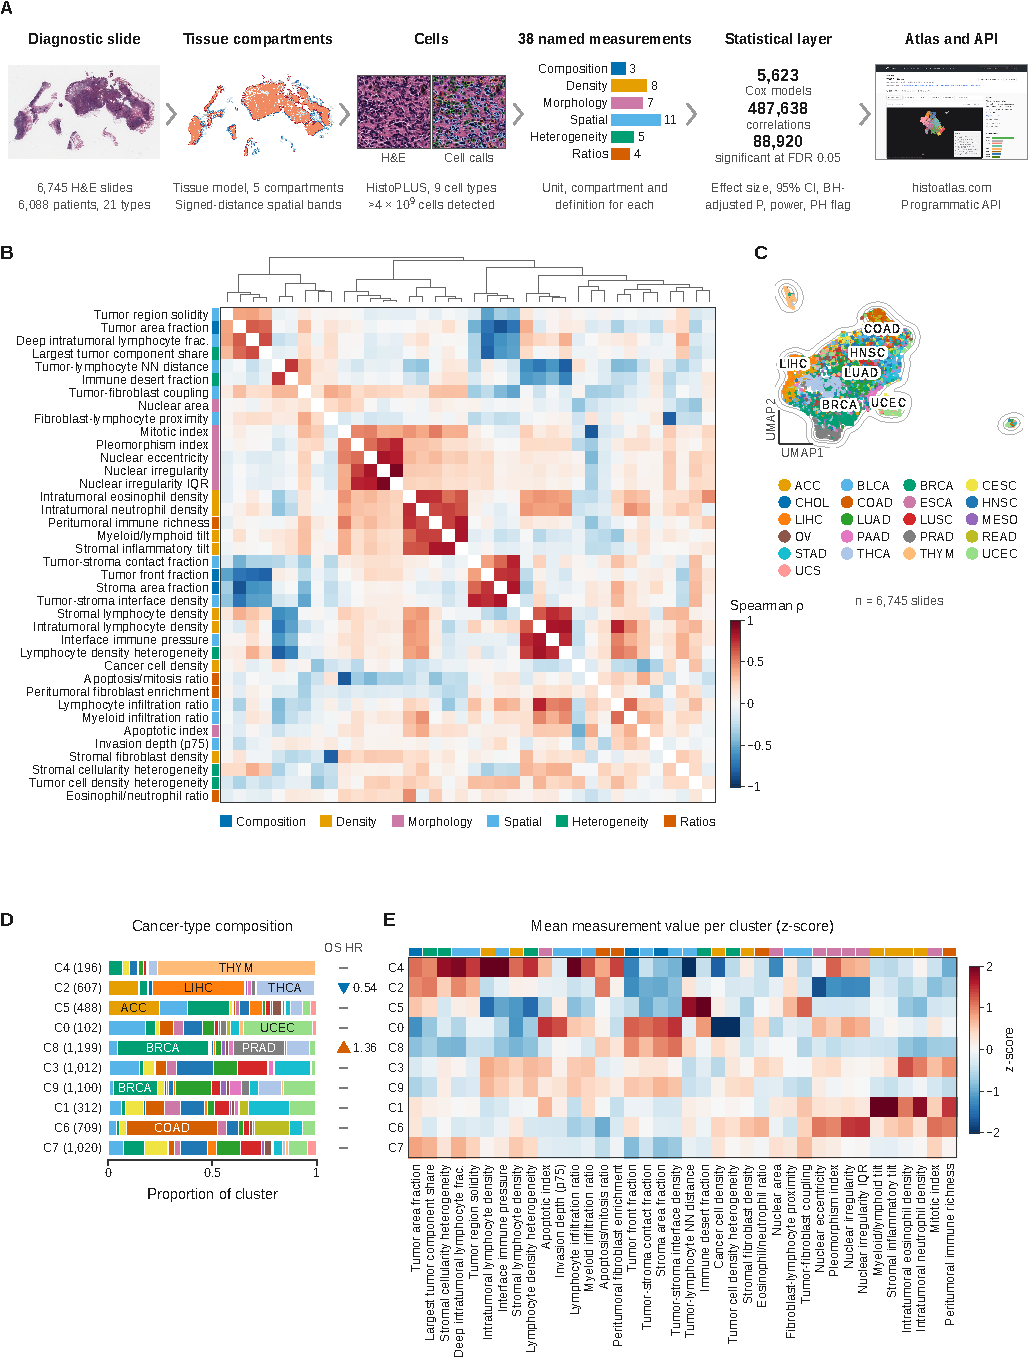
\includegraphics[width=\textwidth,height=0.92\textheight,keepaspectratio]{Figure1.pdf}\\[4pt]\textbf{Figure 1}\end{center}
\clearpage

\begin{center}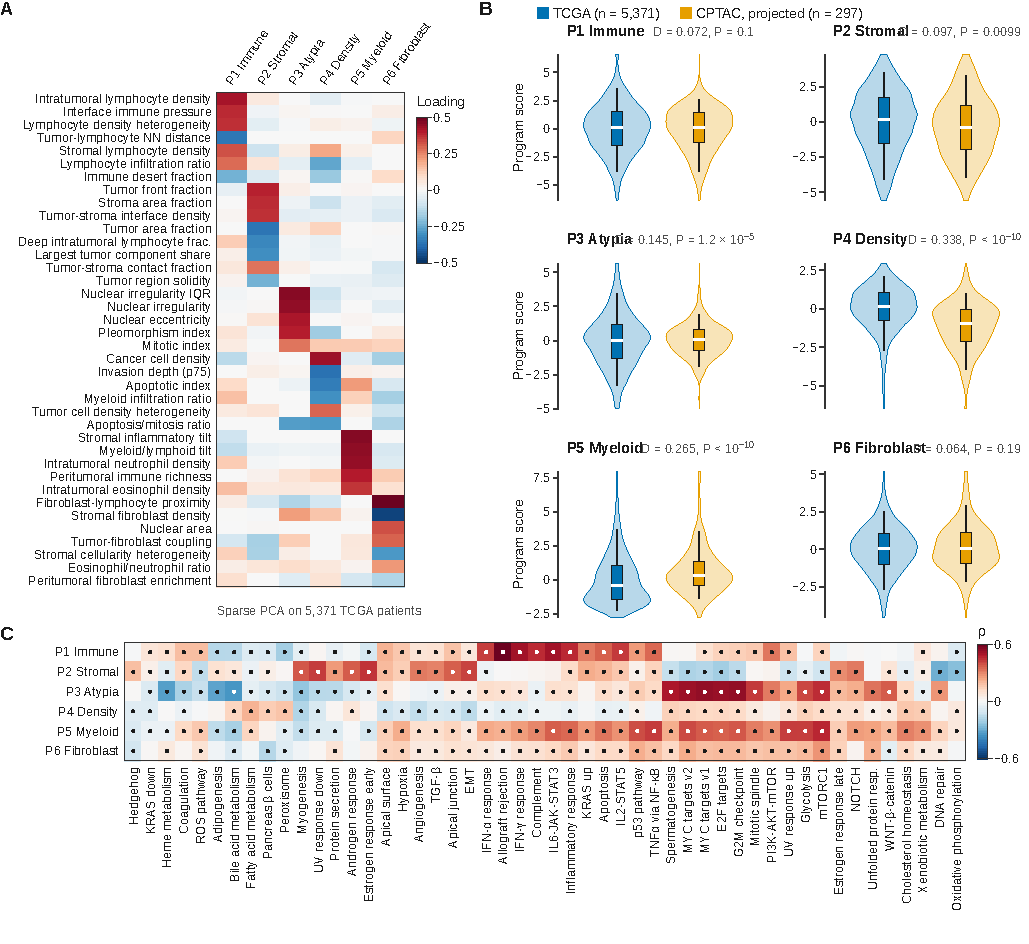
\includegraphics[width=\textwidth,height=0.92\textheight,keepaspectratio]{Figure2.pdf}\\[4pt]\textbf{Figure 2}\end{center}
\clearpage

\begin{center}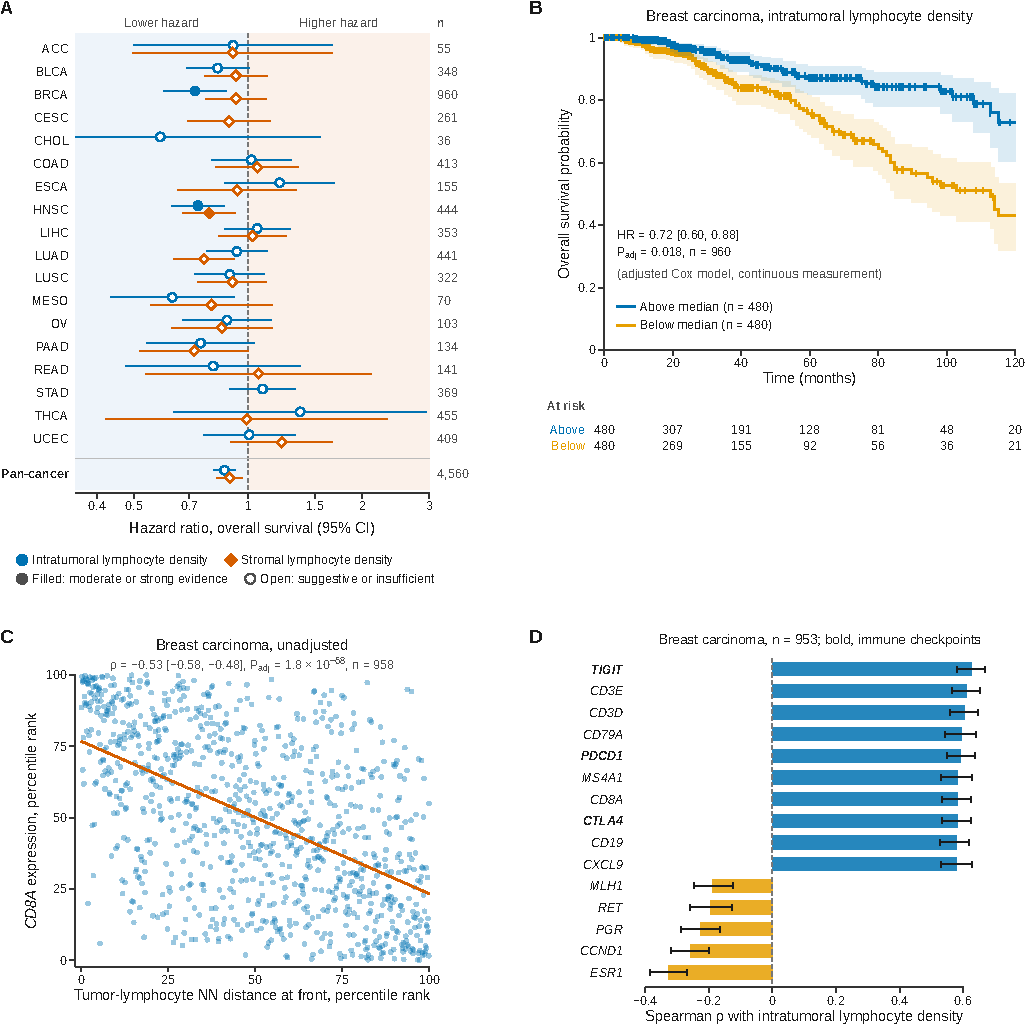
\includegraphics[width=\textwidth,height=0.92\textheight,keepaspectratio]{Figure3.pdf}\\[4pt]\textbf{Figure 3}\end{center}
\clearpage

\begin{center}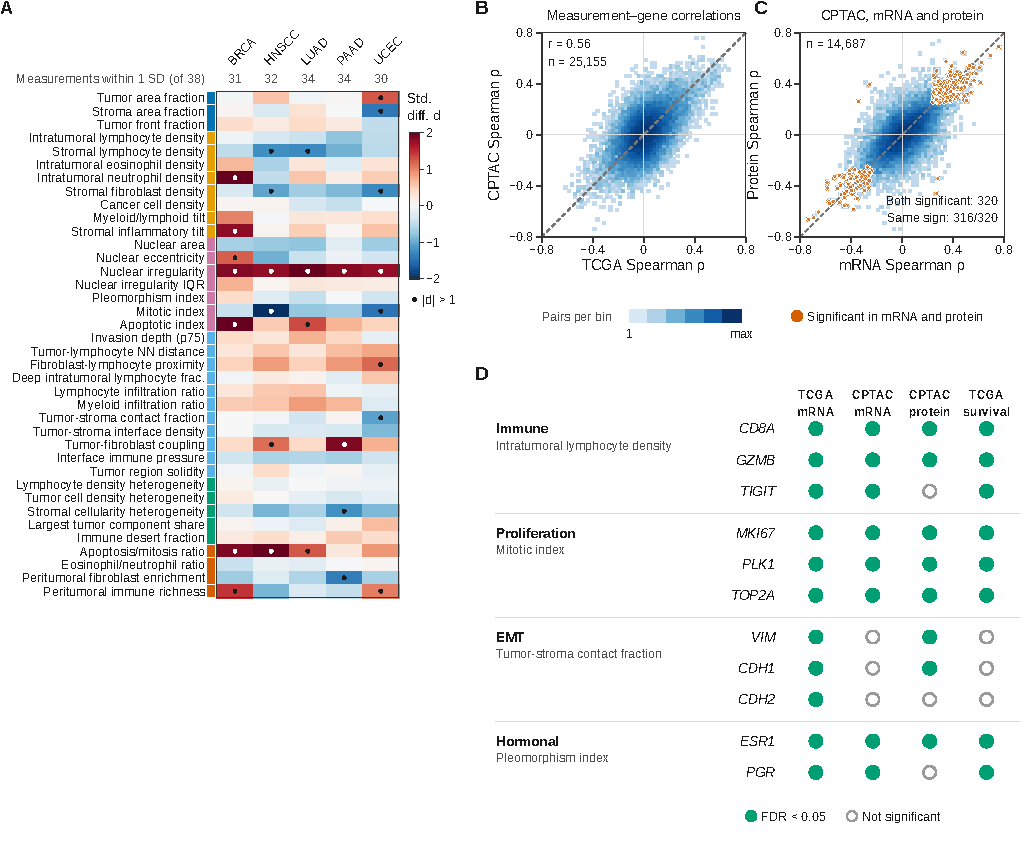
\includegraphics[width=\textwidth,height=0.92\textheight,keepaspectratio]{Figure4.pdf}\\[4pt]\textbf{Figure 4}\end{center}
\clearpage

\begin{center}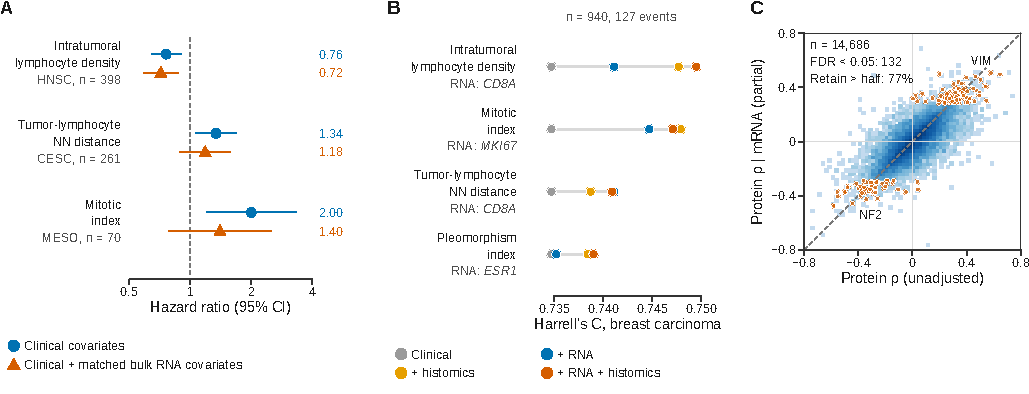
\includegraphics[width=\textwidth,height=0.92\textheight,keepaspectratio]{Figure5.pdf}\\[4pt]\textbf{Figure 5}\end{center}
\clearpage

\begin{center}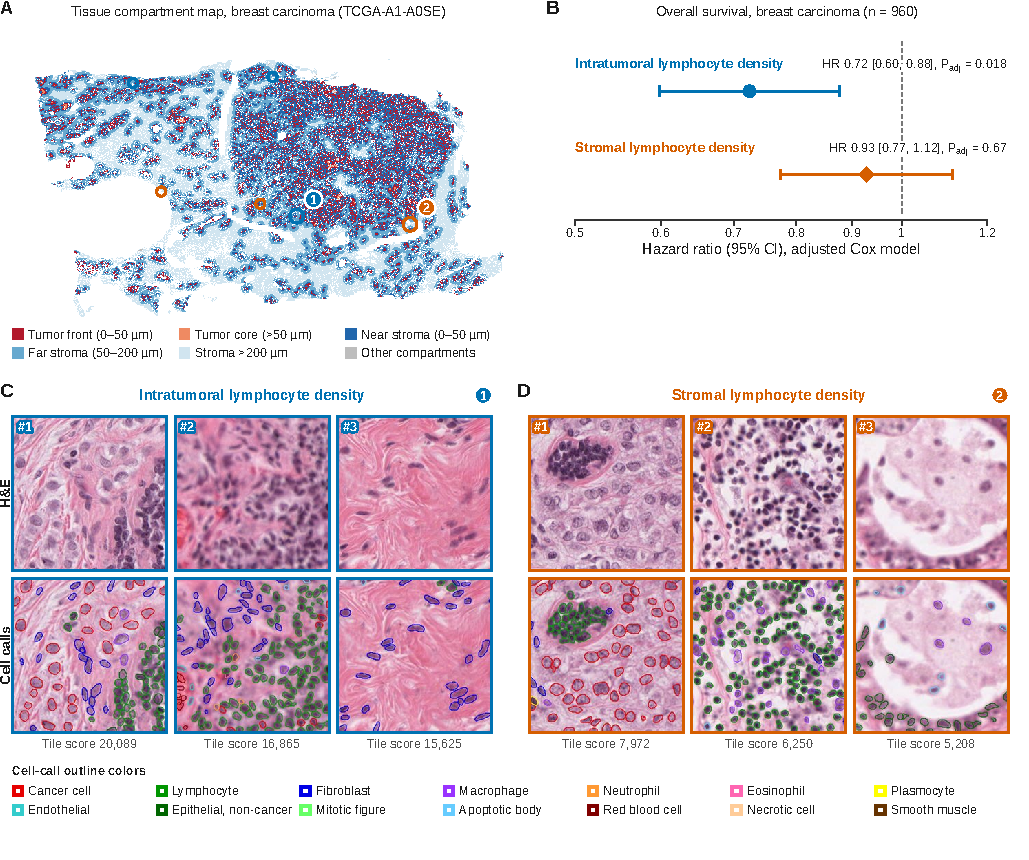
\includegraphics[width=\textwidth,height=0.92\textheight,keepaspectratio]{Figure6.pdf}\\[4pt]\textbf{Figure 6}\end{center}
\clearpage
